%%%%%%%%%%%%%%%%%%%%%%%%%%%%%%%%%%%%%%%%%%%%%%%%%%%%%%%%%%%%%%%%%%%%%%
%% Fintroduction.tex
%% Description:   
%% Author:        Carsten Wulff <wulff@iet.ntnu.no>
%% Created at:    Thu Apr 24 16:32:35 2008
%% Modified at:   Wed Oct 29 19:44:58 2008
%% Modified by:   Carsten Wulff <wulff@iet.ntnu.no>
%%%%%%%%%%%%%%%%%%%%%%%%%%%%%%%%%%%%%%%%%%%%%%%%%%%%%%%%%%%%%%%%%%%%%%
\chapter{Introduction}\label{sc:intro}


How can we make efficient analog-to-digital converters (ADCs) in nano-scale
CMOS?
Challenges like reduced headroom and reduced output resistance has
made it hard to design efficient ADCs in the new nano-scale CMOS technologies.
Why do we want more efficient ADCs? The simple answer is: longer
battery life. The ADC is a key component in any signal chain that
interface with the real world. The receive chain of GPRS networks, Wi-Fi
networks, indeed any current mobile wireless communication technology has an
ADC. Most of the processing today is done in the digital
domain. The pure analog signal chains have been banished to obscurity. But the real world
is analog, and information from the real world must be converted to
digital before it can be digitally processed.

Consumers demand high speed mobile networking on 
the bus to work, at the local cafe, and in their homes. They want 
their portable devices
to have infinite battery lives, and they should cost nothing. 
To
reduce the cost and increase efficiency there has been a push for
integration of features on a single chip (System-on-Chip). 
In SoCs with high integration most of the functions are digital, thus
technologies that allow cheap integration of digital features are
used. These are the nano-scale technologies (less than 100nm
transistor gate length). 

%Two of the challenges that face an analog
%designer in nano-scale CMOS are: reduced headrom, and reduced output resistance.


%\n{Reduced headroom}
Reliability concerns of downscaled CMOS transistors has lead to a
decrease in power supply. At high electrical fields the transistor
gate oxide breaks down. In downscaled transistors the thickness of
the gate oxide is reduced, hence the maximum power supply  must be
reduced. Fig. \ref{fig:supplyscaling} shows the historic power supply  and
  future trends (from ITRS 2007 \cite{itrs07}). At the 250nm gate
  length the power supply is 2.5V, but in 90nm  the power supply
  is reduced to 1.2V.

A challenge with reduced power supply is the reduced signal swing, 
in most cases the signal swing cannot be larger than the power supply.
The accuracy of an ADC is proportional to sampling
capacitance\footnote{This is easily seen from the equation
\eqn{
  S/R = \frac{Signal\:Power}{Noise\:Power} = \frac{A^2/2}{kT/C} = \frac{A^2 C}{2kT}
}}, and
sampling capacitance is inversely proportional to the square of the
signal swing.
 Hence, the capacitor
  size quadruples when we go from 250nm to 90nm CMOS
  technology for the same accuracy. An increased
  capacitor size result in higher area consumption and increased cost.
\begin{figure}[htbp]
\centerline{ 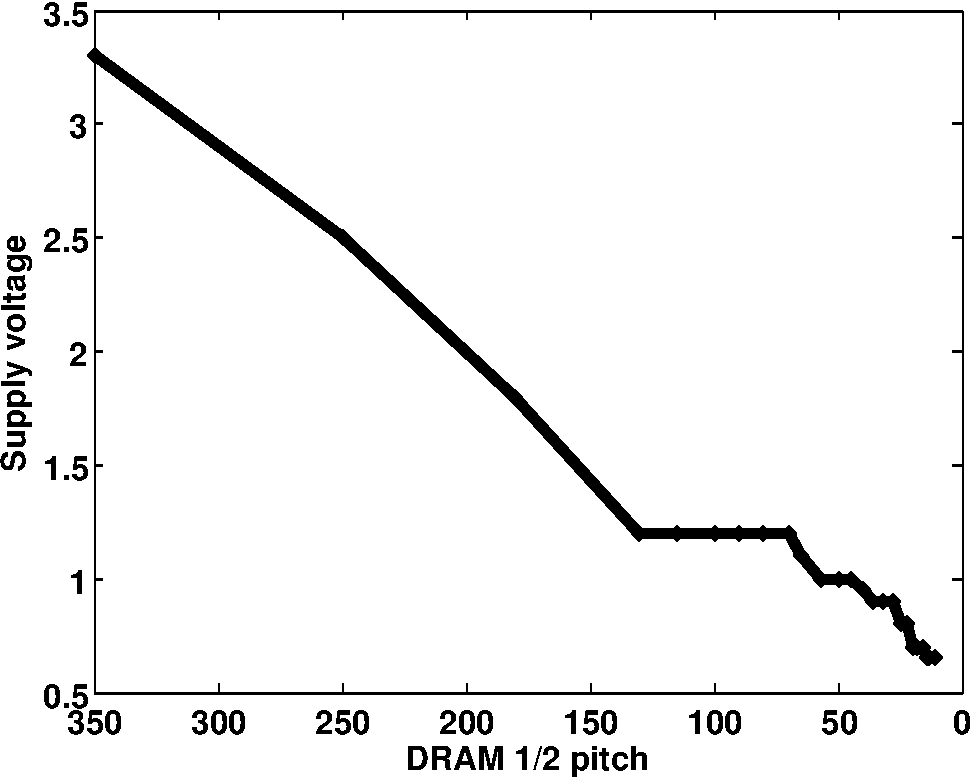
\includegraphics[width=\myfigwidthb]{graphics/supplyscaling}}
  \caption{Historic and future 
    scaling of power supply (based on ITRS 2007
    \cite{itrs07}). DRAM 1/2 pitch is smallest half-pitch of
  contacted metal lines in a DRAM cell.} 
  \label{fig:supplyscaling}
\end{figure}


%\subsection{Reduced output resistance} 
Another challenge is the reduced output resistance of nano-scale CMOS transistors.
  As devices are scaled down the
  transistor channel lengths  shorten. At shorter channel lengths channel
  length modulation and drain induced barrier lowering \cite{troutman79} reduce the output resistance of the
  transistor. Longer channels can be used to increase
  the output resistance, but the effectiveness of using a longer channel is reduced by the pocket
  implants \cite{cao99}. Pocket implants are used to reduce $V_T$ roll-off and
  punch-through in nano-scale technologies. 
%At longer channel lengths the pocket
%  implants cause a drain induced threshold shift (DITS).
% The impact of
%  the pocket implants depend on their dosing concentration, a higher
%  dose lead to a lower output resistance.  
Due to the pocket implants the output resistance of a 1$\mu$m long
  transistor in a 90nm technology is lower than a 1$\mu$m long transistor in
  a 350nm technology.

For high accuracy circuits we need high gain in our transistors. The
gain in a transistor is proportional to the output resistance of the
transistor. The gain of the single transistor is called the intrinsic
gain. 
%The output resistance influence the intrinsic gain of a transistor.
%Longer channels can be used to increase output
%  resistance, but the drain-induced
%  threshold shift (DITS) caused by the pocket implant used in
%  nano-scale technologies 
%  The 
%  intrinsic gain is a measure of how much gain we can
%  expect from one transistor. 
It is
  defined as $A_i =  g_m/g_{ds}$, where $g_m$ is the transconductance
  and $g_{ds}$ is the output conductance (inverse of output
  resistance). 
  When the output resistance is reduced the intrinsic gain
  goes down, and in 65nm technology the intrinsic gain of a minimum
  device is 6\footnote{$L=0.06$, $W=10L$, $V_{DS}=V_{DD}/2$,
    $V_{EFF} = V_{DD}/8$, typical corner} (15-dB). In 350nm technology a minimum 
  device has a gain of 43\footnote{$L=0.35$, $W=10L$, $V_{DS}
    = V_{DD}/2$, $V_{EFF} = V_{DD}/8$, typical corner} (32-dB). As a result, one must use multiple
  stages, cascoding, or gain boosting to achieve high gain amplifiers
 in 65nm technology. But techniques like cascoding (stacking
 transistors) is hard in 65nm technology due to the low supply
 voltage. 
%\end{description}

Downscaling of analog circuits is not all bad. The speed can be
increased due to shorter channel lengths, and the parasitic
capacitances are smaller. But these two advantages are overshadowed by
the reduction in gain and power supply.


We believe that efficiency in nano-scale technology is best attacked
from both ends: the circuit implementation, and the ADC architecture.


One approach to efficiency is to investigate the architectural level. If we
assume that the circuit challenges can be solved, can we do anything
about the ADC architectures? High
accuracy (14-bit) high-speed ($>$ 10MS/s) ADCs are challenging to
implement in nano-scale technologies because of the large sampling
capacitors. With a 1V input
signal swing the
sampling capacitors will be 53pF for a 14-bit converter, which is a
large capacitor. To reduce the sampling capacitor we can use
oversampling. In sigma-delta modulators oversampling is used in
addition to quantization noise shaping to achieve high
accuracy. We wanted to investigate a class of sigma-delta modulators
called \textit{Open-Loop Sigma-Delta Modulators} (OLSDM), and their
use as a front-end to pipelined ADCs. The part of this thesis that
focus on OLSDM is of a theoretical nature.

The other approach to increased efficiency is to investigate the
circuit implementation. 
Switched-capacitor (SC) circuits are ubiquitous in ADCs. They are a tried
and tested accurate method of implementing  high speed
ADCs. The sigma-delta modulators and pipelined ADCs predominate in
the use of SC circuits. The traditional approach to SC  circuits use
opamps, which consume most of the
power in an ADC. In nano-scale technology opamps have become
increasingly hard to design due to the reduced headroom and decreased
output resistance. Techniques that replace opamps have received
interest from the research community. Part of this thesis investigate
how one can replace opamps in pipelined ADCs, and through
this improve efficiency. This part of the thesis is a combination of
theoretical work and measurements on a nano-scale CMOS ADC. 


\section{Main contributions}
The main contributions of this thesis are:


%\subsection{Efficient architectures for pipelined ADCs}
\begin{itemize}
\item We introduce the switched-capacitor modulo integrator. It facilitates
  implementation of switched-capacitor open-loop sigma-delta
  modulators.
\item We introduce the switched-capacitor open-loop sigma-delta
  modulator. A versatile type of sigma-delta modulator suited as
  front-end to pipelined ADCs
\item We introduce the modulo resonator. It enables implementation of high
  resolution open-loop sigma-delta modulators with low oversampling ratio.
\item We prove that open-loop sigma-delta modulation is equivalent to
  sigma-delta modulation if
\eqn{
  |x_n| < R\left(\frac{1}{2} - \frac{2^{N-1}}{2^B}\right)
}
where $x_n$ is the input signal at time $n$, $R$ is the full scale
range, $N$ is the order of the modulator and $B$ is the number of bits in
the quantizer.
\item We introduce the switched open-loop residue amplifiers. Using these the power
  dissipation is reduced by 23\% for a  7-bit pipelined ADC.
\item We introduce the first fully differential silicon proven comparator-based
  switched-capacitor pipelined ADC. Differential implementation allow
  higher signal swing, which is essential
  in nano-scale technologies.

\end{itemize}
Other significant contributions are:

\begin{itemize}

\item We present a comprehensive figure of merit survey of ADCs in Journal of Solid State
  Circuits (1975-2008) and
  International Solid State Circuits conference (2000-2008).
\item We present the  limits of figure of merit for ADCs
\item We present design equations for comparator-based
  switched-capacitor circuits.
\item We introduce a simple calibration scheme for comparator threshold
  calibration. This technique cancels the overshoot in
  comparator-based switched-capacitor pipelined ADCs

\end{itemize}

%\end{enumerate}

%\subsection{Open-Loop Sigma-Delta Modulators}
%\begin{enumerate}




\section{Thesis outline}
This thesis is a collection of papers, hence the 
results are in the papers. The research presented in this thesis is on analog-to-digital
converters, with focus on pipelined ADCs and sigma-delta modulators. If this subject is unfamiliar we suggest reading 
Chapters 9, 10, 11, 13 and 14  in \cite{johns}. 
%For your convenience we have included an introduction
%to ADCs in 
%(Appendix \ref{ap:primer}) and  an introduction to the mathematics of noise sources
%(Appendix \ref{ap:noise}).


This thesis is organized as follows: Chapter \ref{sc:limits} discuss
the fundamental limits of ADC figure of merit, and how parasitic
capacitance make it hard to implement a low resolution converter with
high efficiency.

In Chapter \ref{sc:research} the papers are introduced and we detail how the papers are related. 
The papers are presented in Chapter \ref{sc:p1} to Chapter
\ref{sc:p7}. Comments to papers, a conclusion and further work is
presented in Chapter \ref{sc:remarks}

%In Chapter \ref{sc:papers} the papers are presented.


%%% Local Variables: 
%%% mode: latex
%%% TeX-master: "../../wulff/work/ntnu/phd/thesis/tb_introduction"
%%% End: 
